\section{RT-level FSMD-style Implementation - Task 2}

\subsection{System block diagram}

The complete top-level system is shown in Figure~\ref{fig:gcd-top-block}.
The top-level entity \texttt{gcd\_top} (architecture \texttt{fsmd\_io}) passes the request through the entity \texttt{debounce} (architecture \texttt{behavioral}) before it reaches the entity \texttt{gcd} (architecture \texttt{fsmd}), which contains the controller and the datapath. The debouncer's \texttt{db\_tick} output is left unconnected.

% Block diagram 
\begin{figure}[ht]
\begin{center}
    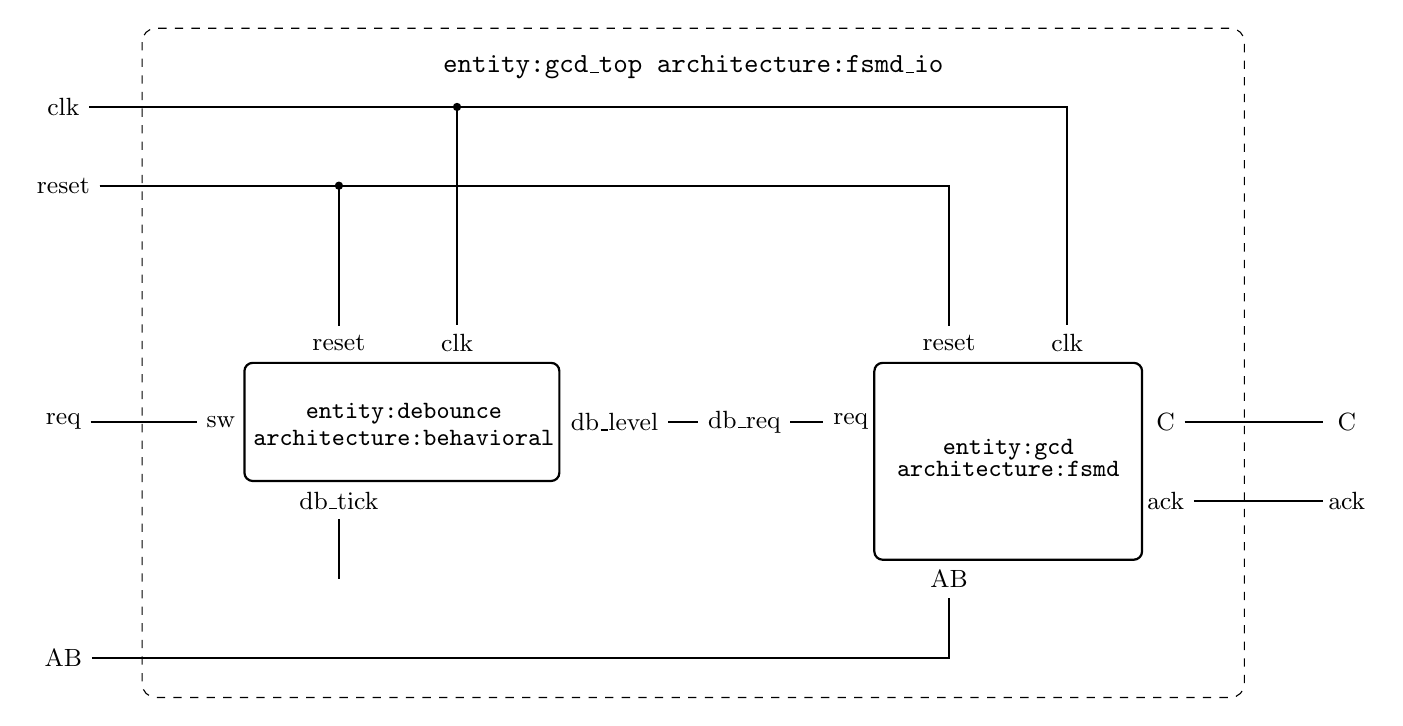
\begin{tikzpicture}[]
        \node[font=\small] (clk_gcd_top)   at (0, 6) {clk};
        \node[font=\small] (reset_gcd_top) at (0, 5) {reset};
        \node[font=\small] (req_gcd_top)   at (0, 2) {req};
        \node[font=\small] (AB_gcd_top)    at (0, -1) {AB};
        \node[font=\small] (clk_db)     at (5, 3) {clk};
        \node[font=\small] (reset_db)   at (3.5, 3) {reset};
        \node[font=\small] (sw_db)      at (2, 2) {sw};
        \node[font=\small](db_level_db) at (7, 2) {db\_level};
        \node[font=\small](db_tick_db)  at (3.5, 1) {db\_tick};
        \node[font=\small] (db_req) at (8.65, 2) {db\_req};
        \node[font=\small] (clk_gcd)   at (12.75, 3) {clk};
        \node[font=\small] (reset_gcd) at (11.25, 3) {reset};
        \node[font=\small] (req_gcd)   at (10, 2) {req};
        \node[font=\small] (AB_gcd)    at (11.25, 0) {AB};
        \node[font=\small](C_gcd)       at (14, 2) {C};
        \node[font=\small](ack_gcd)     at (14, 1) {ack};
        \node[font=\small](C_gcd_top)   at (16.3, 2) {C};
        \node[font=\small](ack_gcd_top) at (16.3, 1) {ack};

        \draw[thick, rounded corners=3pt] (2.3,2.75) rectangle (6.30,1.25) {};
        \draw[thick, rounded corners=3pt] (10.3,2.75) rectangle (13.70,0.25);
        \draw[dashed, rounded corners=5pt] (1,7) rectangle (15,-1.5);

        \fill[thick] (5,6) circle (1.5pt);
        \fill[thick] (3.5,5) circle (1.5pt);

        \node[] at (4.325, 2.1) {\small{\texttt{entity:debounce}}};
        \node[] at (4.325, 1.8) {\small{\texttt{architecture:behavioral}}};
        \node[] at (12, 1.65) {\small{\texttt{entity:gcd}}};
        \node[] at (12, 1.4) {\small{\texttt{architecture:fsmd}}};
        \node[] at (8, 6.5) {\texttt{entity:gcd\_top  architecture:fsmd\_io}};
        
        \draw[-, thick] (req_gcd_top) -- (sw_db);
        
        \draw[-, thick] (clk_gcd_top) -| (clk_db);
        \draw[-, thick] (clk_gcd_top) -| (clk_gcd);
        \draw[-, thick] (reset_gcd_top) -| (reset_db);
        \draw[-, thick] (reset_gcd_top) -| (reset_gcd);
        \draw[-, thick] (AB_gcd_top) -| (AB_gcd);

        \draw[-, thick] (db_level_db) -- (db_req) -- (req_gcd);

        \draw[-, thick] (db_tick_db) -- (3.5, 0);

        \draw[-, thick] (C_gcd) -- (16, 2);
        \draw[-, thick] (ack_gcd) -- (16, 1);
    \end{tikzpicture}
\caption{Top-level block diagram of the GCD system, showing entity and architecture names.}
\label{fig:gcd-top-block}
\end{center} 
\end{figure}


\subsection{State diagram}

In Figure~\ref{fig:gcd_fsm} the final state diagram has been modeled using the state diagram fragment given in the assignment specifications document. It is worth noting that, as required by the assignment, the state bubbles are annotated with RT operations instead of individual control signals, which are listed in Table~\ref{tab:fsm_controls}. Similarly, the asynchronous \texttt{reset} forces the FSM into state \texttt{RST} from any state and is omitted from individual transitions for clarity. The output value C is 0 in every state except DONE, where C <= RegA. The FSM is a Moore machine: all the outputs (\texttt{ack}, \texttt{C} and the register updates) are associated with the states, while the transitions carry only conditions on the input \texttt{req} and on the comparison of $A$ and $B$, which is evaluated through the flags $Z$ and $N$.


\begin{figure}[H]
    \centering
    \begin{adjustbox}{max width=\linewidth}
    \begin{tikzpicture}[
        >={Stealth[round]},
        every state/.style={draw, thick, minimum size=30mm, inner sep=1pt, font=\scriptsize, align=center},
        every edge/.style={draw, ->, thick},
        lbl/.style={font=\footnotesize, align=center},
      ]
        % ---------- states (RT operation performed in each state written inside the circle) ----------
        % Riga superiore
        \node[state, initial above, initial text=] (RST) at (0,0) {\textbf{RST}};
        \node[state] (FHS) at (5.4,0)  {\textbf{FIRST\_HS} \\[6pt]
            \footnotesize RegA <= AB};
        \node[state] (AST) at (10.8,0) {\textbf{A\_STORED} \\[6pt]
            \footnotesize ack $=1$\\};
        \node[state] (WU)  at (16.2,0) {\textbf{WAIT\_USER}};

        % Riga centrale
        \node[state] (SHS) at (16.2,-7.5) {\textbf{SECOND\_HS} \\[6pt]
            \footnotesize RegB <= AB};
        \node[state] (CMP) at (10.8,-7.5) {\textbf{COMPUTE}};
        \node[state] (CHK) at (5.4,-7.5)  {\textbf{CHECK\_ZERO}};
        \node[state] (DN)  at (0,-7.5)    {\textbf{DONE} \\[6pt]
            \footnotesize ack $=1$ \\ \footnotesize C <= RegA};

        % NEG sopra, POS sotto: stessa x, a meta' tra CHECK_ZERO e COMPUTE
        \node[state] (NEG) at (8.1,-4.9)  {\textbf{NEG} \\[6pt]
            \footnotesize RegB <= RegB $-$ RegA};
        \node[state] (POS) at (8.1,-10.1) {\textbf{POS} \\[6pt]
            \footnotesize RegA <= RegA $-$ RegB};

        % ---------- transitions ----------
        \path
          (RST) edge[loop left]     node[lbl, left]  {req $=0$} ()
          (RST) edge                node[lbl, above] {req $=1$} (FHS)
          (FHS) edge                (AST)
          (AST) edge[loop above]    node[lbl, above] {req $=1$} ()
          (AST) edge                node[lbl, above] {req $=0$} (WU)
          (WU)  edge[loop above]    node[lbl, above] {req $=0$} ()
          (WU)  edge                node[lbl, right] {req $=1$} (SHS)
          (SHS) edge                (CMP)
          (CMP) edge                (CHK)
          % NEG: archi curvi verso l'esterno (sopra)
          (CHK) edge[bend left=25]  node[lbl, above, sloped] {$A<B$} (NEG)
          (NEG) edge[bend left=25]  (CMP)
          % POS: archi curvi verso l'esterno (sotto)
          (CHK) edge[bend right=25] node[lbl, below, sloped] {$A>B$} (POS)
          (POS) edge[bend right=25] (CMP)
          (CHK) edge                node[lbl, above] {$A=B$} (DN)
          (DN)  edge[loop left]     node[lbl, left]  {req $=1$} ()
          (DN)  edge                node[lbl, right] {req $=0$} (RST);

    \end{tikzpicture}
    \end{adjustbox}
    \caption{State diagram of the GCD FSM.}
    \label{fig:gcd_fsm}
\end{figure}


\subsection{Implementation}

The fsmd architecture separates datapath and control into dedicated sequential and combinational blocks: a single clocked process (\texttt{seq}) handles the state register and datapath registers (\texttt{reg\_a}, \texttt{reg\_b}), while combinational logic is partitioned between the FSM controller (\texttt{cl\_fsm}) and dedicated datapath units (\texttt{cl\_mux}, \texttt{cl\_calc} and \texttt{cl\_eval}).


We decided to follow the essential rules of the assignment suggested template by keeping a strict separation between combinational logic and flip-flops: \texttt{seq} is the only clocked process and contains all and only the flip-flops, while every other process is purely combinational and starts with default assignments. What we changed is that the single combinational process is split into the blocks of Figure~\ref{fig:basic-fsmd}, i.e.\ the controller, the multiplexer, the ALU and the flag evaluation. We consider this an improvement because each process maps one-to-one onto a box of Figure~\ref{fig:basic-fsmd}, so the code can be checked against the figure and the state diagram by inspection, and the register enables \texttt{LDA} and \texttt{LDB} are used directly instead of the \texttt{next\_RegA}/\texttt{next\_RegB} signals of the template, which would only duplicate them. Each process also has a short sensitivity list and a single responsibility, whereas a single process containing the FSM, the multiplexer and the arithmetic would need a large sensitivity list that is easy to get incomplete, and would hide the datapath inside the \texttt{case} statement of the controller. 

The controller \texttt{cl\_fsm} realizes the register transfers of Figure~\ref{fig:gcd_fsm} by driving the control signals of Figure~\ref{fig:basic-fsmd}; their values in each state are listed in Table~\ref{tab:fsm_controls}.

\begin{table}[H]
    \centering
    \footnotesize
    \renewcommand{\arraystretch}{0.9}
    \begin{tabular}{lcccccc}
        \toprule
        State & \texttt{ABorALU} & \texttt{LDA} & \texttt{LDB} & \texttt{FN} & \texttt{ack} & \texttt{C} \\
        \midrule
        \texttt{RST}        & 0 & 0 & 0 & 00 & 0 & 0 \\
        \texttt{FIRST\_HS}  & 1 & 1 & 0 & 00 & 0 & 0 \\
        \texttt{A\_STORED}  & 0 & 0 & 0 & 00 & 1 & 0 \\
        \texttt{WAIT\_USER} & 0 & 0 & 0 & 00 & 0 & 0 \\
        \texttt{SECOND\_HS} & 1 & 0 & 1 & 00 & 0 & 0 \\
        \texttt{COMPUTE}    & 0 & 0 & 0 & 00 & 0 & 0 \\
        \texttt{CHECK\_ZERO}& 0 & 0 & 0 & 00 & 0 & 0 \\
        \texttt{POS}        & 0 & 1 & 0 & 00 & 0 & 0 \\
        \texttt{NEG}        & 0 & 0 & 1 & 01 & 0 & 0 \\
        \texttt{DONE}       & 0 & 0 & 0 & 10 & 1 & \texttt{RegA} \\
        \bottomrule
    \end{tabular}
    \caption{Control signals of the FSM in each state.}
    \label{tab:fsm_controls}
\end{table}

Within the datapath, the ALU (\texttt{cl\_calc}) extends the 16-bit register operands with a leading zero to perform arithmetic over a 17-bit signed range. Using a 17-bit ALU rather than a 16-bit one ensures that unsigned 16-bit values fit into the positive dynamic range of two's-complement arithmetic, preventing overflow and allowing negative results to be detected directly via the most significant bit, without requiring dedicated carry logic. 

The interface uses a four-phase handshake protocol to synchronize transactions: ack is asserted in \texttt{A\_STORED} and \texttt{DONE} and remains asserted until req is cleared by the user. Furthermore, the output port \texttt{C} is held at zero across all intermediate states and is assigned to \texttt{reg\_a} exclusively during \texttt{DONE}. Because the FSM transitions from \texttt{DONE} back to \texttt{RST} once req drops to '0', the circuit returns to its ready state autonomously.

\subsection{Design verification and test}

% One sentence per line: comment out any line with a leading %.
The testbench provided in Task~1 only contains five operand pairs, so we replaced it with 10\,000 random pairs in the range $[1, 2^{16}-1]$, generated by \texttt{test/test\_generator.py}, with the expected results computed by Python's \texttt{gcd}.
Random pairs with $A>B$ and $A<B$ exercise both \texttt{POS} and \texttt{NEG}, together with the transition to \texttt{DONE}, the waiting loops on \texttt{req}, and many consecutive computations without reset, so every transition of Figure~\ref{fig:gcd_fsm} is taken.
All the assertions pass, and the simulation ends after 47\,720\,260~ns.
Euclid's algorithm as specified in the assignment is defined for positive integers only, so we did not test the edge cases in which an operand is zero. If exactly one of $A$ and $B$ is $0$, the subtraction-based algorithm never terminates, and the circuit would stay in its computation loop until it is reset.

\subsection{Resources used}

Table~\ref{tab:t2_resources} compares the resources estimated in the subsection ``\nameref{resources-estimate}'' with the synthesis report of the \texttt{gcd} module.

\begin{table}[H]
    \centering
    \small
    \begin{tabular}{lcc}
        \toprule
        Resource & Estimated (Task~0b) & Synthesized \\
        \midrule
        FFs                        & 32 & 36 \\
        LUTs                       & 35 & 69 \\
        \bottomrule
    \end{tabular}
    \caption{Estimated vs.\ synthesized resources.}
    \label{tab:t2_resources}
\end{table}

\begin{itemize}
    \item \textbf{FFs:} the number of estimated flip-flops matches the synthesized one if we include the control part. In fact, the FSM has 10 states which need 4 additional FFs.
    \item \textbf{LUTs:} in this case, the number of synthesized LUTs is significantly higher than the estimated one. This discrepancy occurs because the previous estimation did not account for several hardware components of the complete design; specifically, the FSM logic, the output gating for C, and the 17-bit ALU.
\end{itemize}